\begin{savequote}[75mm]
Nothing in Biology Makes Sense Except in the Light of Evolution
\qauthor{Theodosius Dobzhansky}
\end{savequote}

\chapter{Introduction}
\label{introduction}
\begin{flushleft}
\setlength{\parindent}{7ex}
\section{Disclosure}
Parts of this introduction, especially the section on Wnt signaling, have been adapted from own publications, including \textit{Wnt signaling in cancer} \cite{Zhan2017}

\section{Colorectal Cancer}

Colorectal Cancer is among the three most common and lethal forms of cancer in the developed world, accounting for ca. 10\% of all cancer incidence and mortality \cite{sungGlobalCancerStatistics2021}. The majority of colorectal cancer cases are diagnosed after the age of 50, are located in a region spanning the rectum and sigmoid colon, and develop from macroscopic precursor lesions referred to as adenomas over the course of ca. 10 years \cite{Cho1992}. Next to patient age, a sedentary lifestyle including obesity, diabetes, consumption of red and processed meats, alcohol and smoking constitute risk factors \cite{sungGlobalCancerStatistics2021}. The disease is classified by the Union for International Cancer Control (UICC) into five stages ranging from \textit{carcinoma-in-situ} (patch of malignant cells that has not yet breached the basal lamina of the intestinal mucosa), to stages 1 (malignant cells have breached the basal lamina), stage 2 (malignant cells have spread beyond the large muscle layer surrounding the colon mucosa), stage 3 (malignant cells have spread to loco-regional lymph nodes), and stage 4 (metastatic disease) \cite{ColorectalCancerStages2012}.\par

Among the most effective interventions to reduce the incidence and mortality of colorectal cancer is the removal of macroscopic lesions during preventative colonoscopy \cite{Nishihara2013Long-TermEndoscopy}. In case the disease has further progressed, therapeutic options include oncological resection coupled with adjuvant chemotherapy (available for UICC 2, recommended for UICC 3) based on the DNA replication inhibitors 5-Fluoruracil (5FU) and Oxaliplatin (FOLFOX). Additional treatment options exist for patient subgroups such as rectal cancer patients (neoadjuvant radiochemotherapy) and frail patients (5FU instead of FOLFOX for adjuvant chemotherapy). In case of metastatic disease (UICC 4) the treatment depends on molecular characteristics of the tumor. Commonly available options include (1) combination chemotherapy (FOLFOX or FOLFIRI) paired with anti-EGFR antibodies (Cetuximab) for KRAS wildtype disease \cite{vancutsemESMOConsensusGuidelines2016a}, (2) triple therapy (FOLFOXIRI \cite{vancutsemESMOConsensusGuidelines2016a}, or combined EGFR-, MEK- and BRAF-inhibitor treatment \cite{kopetzEncorafenibBinimetinibCetuximab2019}) for BRAF mutant disease, or (3) PD-1 immune checkpoint inhibition (Pembrolizumab, anti-PD1) for tumors with microsatellite instability (MSI+) \cite{PembrolizumabMicrosatelliteInstabilityHigh}. Therapeutic options can be combined with angiogenesis inhibiting therapeutic antibodies (Bevacizumab, anti-VEGFR), especially when patients are not able to undergo a full treatment regiment. Additional lines of therapy can also include agents like Regorafenib and Triflouridin/Tipiracil \cite{vancutsemESMOConsensusGuidelines2016a}. \par

\section{Colorectal Cancer Pathogenesis}

\subsection{The colon crypt}

The sequence of molecular events leading to colorectal cancer, or any cancer in general, are governed by the tissue's stem cell biology \cite{CleversCancerStemCell}. The colon stem cell niche, or crypt, is the source of all epithelial cells lining the colon. Similar to the small intestine, LGR5+ intestinal stemcells are located at the bottom of the crypt and continuously renew the epithelium by proliferating and, through displacement, pushing newly formed cells towards the colon's lumen. This architecture serves multiple purposes, including protection of stem cells and the control of cell fate decisions across the epithelium \cite{cleversIntestinalCryptPrototype2013a}. Multiple developmental pathways, especially Wnt signaling, Notch, BMP and RAS-MAPK signaling, govern cell identity and growth rate in the intestinal niche \cite{Gehart2019}. The concentration of ligands for most of these signaling pathways is organized in gradients along the crypt-lumen axis. For example, the concentration of stem cell identity maintaining Wnt ligands (Wnt signaling) and growth-rate controlling EGF ligands (RAS-MAPK signaling), decreases as cells are pushed outside of the crypt \cite{Sasaki2016}. In contrast, the effect of BMP ligands, which promote cell differentiation, increases as the concentration of BMP inhibitors (i.e. Noggin) derived from basal mesenchymal cells decreases \cite{heBMPSignalingInhibits2004}. As a cell is pushed outside the crypt by a continuous stream of proliferating cells, the signals it receives and with it its gene expression changes - leading to cellular differentiation. Similarly, if enterocyte-progenitors are moved back into the crypt, the ambient signaling leads to a de-differentiation towards an intestinal stem cell state \cite{tettehReplacementLostLgr5Positive2016a}. \par

Given the spacial confinement of growth- and stemness-stimulating signals, the crypt architecture also leads to a protection against tissue damage. At the bottom of the crypt, a neutral competition of proliferating intestinal stem cells leads to the removal of damaged cells that show a reduced proliferation rate relative to population of surrounding stem cells \cite{snippertIntestinalCryptHomeostasis2010a}. Given this neutral competition and the dependence on external signals to proliferate, dysfunctional or transformed cells have a higher likelihood of being removed from the niche unless they acquire a set of molecular alterations that render them independent from niche signals and increase their growth rate. \par

\subsection{The adenoma carcinoma sequence}

Cancer in general, and colorectal cancer in particular, is a disease marked by the accumulation of genetic events in somatic cells, which over time lead to uncontrolled growth and spread beyond the tissue of origin. Both structural and functional genomics experiments have helped identify functional genetic events or "drivers", that cause the transition from controlled to malignant cellular state. A classic model for the sequence of functional events leading to colorectal cancer is known as the adenoma-carcinoma sequence \cite{vogelsteinGeneticAlterationsColorectaltumor1988}. It starts with the activation of the Wnt signaling pathway through loss of the tumor suppressor APC and is followed by the activation of the RAS-MAPK signaling pathway through mutations of the KRAS or BRAF oncogene. Further mutations activating PI3K signaling (i.e. PI3K oncogene, PTEN tumor suppressor) and inhibiting TGF-beta (i.e. SMAD4 tumor suppressor) and TP53-signaling (i.e. TP53 tumor suppressor) complete the transformation from adenoma to invasive carcinoma \cite{fearonMolecularGeneticsColorectal2011}. \par

When simplified, colorectal cancer forms along the adenoma-carcinoma sequence through (I) a common chromosomal instability (ca 80\%) or (II) a DNA-mismatch repair deficiency (ca. 20\%) associated mechanism \cite{Markowitz2009} and \cite{pancioneGeneticEpigeneticEvents2012} (Figure \ref{colon_cancer_progression}). These two forms of tumor development have been associated with characteristic clinical, pathological, and molecular properties. Tumors of the common chromosomal instability phenotype present themselves early as common, non-serrated polyps in the rectum and sigmoid colon. Most tumors are microsatellite stable and have frequent APC truncating mutations coupled with KRAS activating mutations. In contrast, tumors of the DNA-mismatch repair phenotype are frequently present as serrated polyps and more likely to be located in the right colon \cite{Markowitz2009}. These tumors are often marked by a CPG-island methylation phenotype (CIMP) that can lead to the hypermethylation of tumor suppressors and DNA-mismatch repair genes \cite{oginoCpGIslandMethylator2009}. Consequently, these tumors have a higher proportion of microsatellite instability, higher mutational burden, and thus higher immune-cell infiltration. APC mutations are less frequent and if present more likely to be missense than truncating \cite{borowskyRoleAPCWNT2018}. Mutations of the BRAF oncogene are more frequently found than KRAS mutations. Independent of the mechanism, the sequential accumulation of functional genetic events renders colorectal cancer cells progressively independent of the organism's tissue control mechanisms and thus enable the uncontrolled, tissue independent growth of cells which is associated with late stage cancer.

\subsection{APC and KRAS mutations during colorectal cancer formation}
two mutations that are freuent, highly correlated and found in adenomas. As a result have been  the first two functional events in the adenoma carcinoma sequence. 
Understanding the interaction between the two alleles is an open question - cite Dow

cite Mina - structural evidence for coupling
Of note APC truncating mutations are associated with KRAS, but not with BRAF - an alternative oncogene within the RAS-MAPK pathway which occurs in a an oncogenic state in a mutually exclusive pattern with activated KRAS. When both mutations are present - oncogene induced senescence. 
Also mutation of either KRAS and BRAF alone leads to oncogene induced senescence

functional evidence for coupling
colon organoids - 
mouse studies 

neither apc and kras are individually necessary and sufficient 
apc is necessary for both KRAS context AND KRAS + TP53 - lucas dow

Myc






Coupling of genotypes

A limited set of signaling pathways both control the cell state in the colon stem cell niche and are frequently altered during tumorigenesis. These pathways include (i) Wnt signaling, (ii) ERK MAPK signaling \citep{gehartTalesCryptNew2019}. In the following section the mechanism of Wnt signaling and ERK MAPK signaling are discussed in more detail, as these two pathways are altered by Apc loss and Kras activation, respectively.


While targeted inhibitors for mutant KRAS and BRAF have been developed, APC currenlty remains an intractable pharmacological target. 

\begin{figure}[h]
\centering
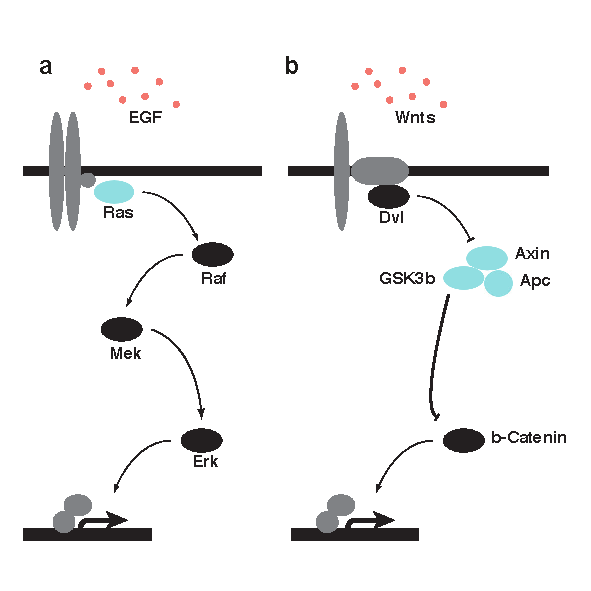
\includegraphics[width=0.55\textwidth,
                keepaspectratio]{figures/adenomaprofiling/pdf/fig_0_1.pdf}
\caption[Simplified illustration of ERK-MAPK signaling and canonical Wnt signaling]{\textbf{Simplified illustration of EGF dependent ERK-MAPK signaling and canonical Wnt signaling a} EGF dependent signaling cascade. Ras is highlighted in blue. \textbf{b} canonical Wnt signaling cascade. The destruction complex, including Apc, is highlighted in blue.}
\label{fig_180}
\end{figure}
\bigbreak


Members of the Wnt signaling pathway were first identified as regulators of embryonic development \cite{Sharma1973WinglessMelanogaster} and are controlling adult stem cell identity across tissues and are thus frequently altered during cancer initiation \cite{Nusslein-Volhard1980MutationsDrosophila}. In canonical Wnt signaling, absence of Wnt ligands leads to phosphorylation of \textbeta-catenin by the destruction complex, which contains the scaffold protein Axin, the large disordered protein APC (Adenomatous polyposis coli) and the kinases GSK3\textbeta as well as casein kinase (CK1\textalpha) (reviewed in Zhan, Rindtorff et al.\cite{Zhan2017}). 
In this state, \textbeta-catenin is phosphorylated by GSK3\textbeta, ubiquitinated by \textbeta-TrCP and subsequently targeted for proteasomal degradation. 
In the absence of nuclear \textbeta-catenin, the transcriptional repressive complex containing TCF/LEF and transducing-like enhancer protein (TLE/Groucho) recruits Histone deacetylases to repress target genes. \par 

The role of Wnt signaling during colorectal cancer development is well established \cite{Polakis2007}. While activating mutations of \textbeta-catenin do exist, loss of APC is the most frequent driver of Wnt signaling in colorectal cancer and can be found in about 80\% of colorectal cancer patients \cite{Fearon1989}. In line with its role as a tumor suppressor, truncating of APC using the CRISPR/Cas9 technology, leads to colorectal cancer development, which can be modeled ex vivo in human intestinal organoids \cite{Matano2015, Drost2015SequentialCells}. Furthermore, by using a mouse model allowing the reversible knockdown of Apc via shRNA, it was demonstrated that adenomas could regress to normal tissue once APC function is restored, establishing that hyper-activated Wnt signaling is necessary for tumor development and maintenance \cite{Dow2015}. 
Although loss of APC in general is a driving event of colorectal cancer development and persistence, not every mutation of the APC gene leads to a similar phenotype. Studies of human colorectal cancer samples and tumors from mouse models revealed that different mutations of APC result in distinct levels of canonical Wnt pathway activity and, in addition, are associated with characteristic tumor locations within the large intestine \cite{Christie2013, Buchert2010}. \par

\subsubsection{ERK MAPK Signaling}

The extracellular-signal-regulated (ERK) mitogen-activated protein kinase family (MAPK) is one of three major MAPK families, together with the JNK (c-jun N-terminal kinase or stress-activated protein kinases) and MAPK14 group of protein kinases. These signaling cascades play a major role in (I) integrating external proliferative signals, (II) reacting to stress or ambient cytokines and (III) protecting cells from apoptosis, respectively \cite{Oncol2005}. 

In the colon crypt, the ERK MAPK signaling cascade and its members Ras-Raf-MEK and ERK are key regulators of cell proliferation. Blockade of EGF, a canonical ligand of the signaling cascade's upstream receptor EGFR, leads to a cell cycle arrest of proliferating Lgr5+ cells while not affecting their cellular state \cite{basakInducedQuiescenceLgr52017a}. As a result of the state preservation, cells can re-enter proliferation as soon as ERK MAPK signaling is restored.

In colorectal cancer, the Ras kinase members are mutated in about 36\% of cases \cite{Oncol2005}. According to the Vogelstein model of colorectal cancer initiation \cite{Fearon1989}, activating mutations of KRAS takes place early during cancer development, more specifically, after loss of APC.
Next to KRAS, BRAF mutations can also be found in around 10\% of colorectal cancers \cite{Oncol2005}. Of note, mutations of KRAS and BRAF occur mostly in a mutually exclusive pattern with BRAF mutations, which are enriched in Microsatellite instable colorectal cancers \cite{Oncol2005, Sahin2013}. 

\subsection{APC and KRAS mutations during colorectal cancer formation}


\section{Organoids}

Organoids are three-dimensional cell culture models from primary adult tissue. Intestinal organoids develop from Lgr5+ adult stem cells and were first isolated from the small intestine of mice \cite{Sato2011}. Subsequently, following the initial publication, further organoid models across tissue-types and species have been developed. These include organoids from intact and cancerous human large intestine \cite{Sato2011}, pancreas \cite{Sachs2017}, mammary epithelium \cite{Zhang2016EstablishingCells, Sachs2017AHeterogeneity} and the hepatobiliary system \cite{Huch2013NIHAccess, Broutier2016CultureManipulation.}. The number of tissues that can be modeled through organoids has been continuously increasing since the first publication of this methodology. \par

Culturing organoids from primary cells requires the addition of specific tissue-dependent growth factors and the embedding of cells in 3D hydrogels \cite{Merker2016GastrointestinalOut}. In the case of colon organoids, the necessary growth factors are inspired by signaling cues available in the intestinal stem cell niche (discussed above): Wnt and R-spondin ligands to activate and maintain canonical Wnt signaling; EGF ligands to stimulate ERK MAPK signaling, and Noggin ligands to inhibit the differentiating effects of the BMP signaling cascade \cite{Sato2013}. When combined with inhibitors of TGF\textbeta and p38 mediated signaling, these growth factors enable organoid formation and continous proliferatation ex-vivo. In line with the niche-focused model of colon cancer formation outlined previously, patient derived colorectal cancer organoids proliferate in simpler conditions that correspond to their genetic state (i.e. APC mutant colon organoids grow in conditions lacking Wnt and R-spondin ligands) \cite{Fujii2016-de}. Not only the high isolation efficiency of up to 80\%, but also the high genetic and transcriptomic correlation with their tissue of origin have made organoids increasingly popular translational research model \cite{pauliPersonalizedVitroVivo2017a}. Both the high isolation efficiency, and the molecular representation of the tissue of origin are likely a result of the culture conditions which are mirroring the tissue-specific stem cell environment. These conditions reduce biases and evolutionary bottlenecks on the tissue's cells during the transfer into an in-vitro environment. \par

\subsection{Diagnostic use of Colorectal Cancer Organoids}

Given the benefits of the methodology, patient derived organoids are being trialed as predictive models for personalised treatment recommendation in colorectal cancer care \cite{VanDeWetering2015, Vlachogiannis2018, ganeshRectalCancerOrganoid2019a, ooftPatientderivedOrganoidsCan2019a, yaoPatientDerivedOrganoidsPredict2020a}. In these assays, personalised organoid models are generated and then treated with a candidate drug in-vitro. While robust reports on the predictive validity of organoids for progression-free survival are still missing, current results for response rate models show considerable predictive validity for Irinotecan, FOLFIRI, and neoadjuvant radiation therapy. A pooled analyses of the previously published literature recently summarised the aggregate sensitivity and specificity for organoid based treatment response rate prediction at 0.81 and 0.74, respectively (conservative single-point AUROC estimate: 0.78) \cite{wensinkPatientderivedOrganoidsPredictive2021, zhangNoteROCAnalysis2005}. For reference, a retrospective study of clinical experts estimated the predictive validity of an emergency room EKG for occlusive myocardial infarction at a sensitivity and specificity of 0.79 and 0.80, respectively (multi-point AUROC estimate: 0.80) \cite{al-zaitiMachineLearningECG2023}. Despite the potential of patient derived organoids to guide clinical decision making, the method is not ready for use in a clinical context with a high biopys-to-evaluation dropout rate and tunraround time being the primary technical hurdles. A recent failed single-arm prospective clinical trial for organoid-based last-line treatment recommendations reported a treatment for 6 out of 61 included patients (>90 \% dropout rate and 10 week turnaround time, 23 lost during organoid establishment, 11 lost due to disease progression) \cite{ooftProspectiveExperimentalTreatment2021}. Further improvements of reagents, isolation procedures, and in-vitro protocols might lead to lower dropout rates and turnaround times to enable further investigation of organoid-based diagnostics for personalised colorectal cancer care. \par

\subsection{Therapeutic Discovery using Colorectal Cancer Organoids}

Next to diagnostics, organoid have been evaluated as models in drug discovery. Patient derived organoids can be processed in high-throughput small molecule screens with conventional cell viability readouts \cite{VanDeWetering2015}. However, besides testing therapeutic candidates on late stage cancer models, organoids are amenable to efficient genetic engineering \cite{Matano2015-zw, Drost2017-fu}. This opens up the possibility of evaluating the effect of therapeutic candidates against precisely defined genetic disease states. For example, organoid models with engineered tumor forming genetic changes, open up searching for therapeutic candidates that show effects specific to a given genetic event. As I will demonstrate throughout this thesis -specifically in the context of multi-genic somatic disease such as colorectal cancer- organoids are promising models for therapeutic discovery programs against (1) early and (2) progressed stages of this disease.

\section{Profiling Experiments} 

Profiling experiments are biological experiments in which high dimensional phenotypes are observed of biological models that are subjected to multiple treatments. Examples for such methods include Transcriptome Profiling Experiments (i.e. Perturb-Seq \citep{dixitPerturbSeqDissectingMolecular2016}, L1000 Profiling \citep{}) as well as Image-based Profiling Experiments \cite{chandrasekaranImagebasedProfilingDrug2021} (described below). These data intensive experiments generate three-dimensional data tensors containing (1) multiple features (i.e. transcript count or morphological feature) for (2) multiple treatments (i.e. small molecules) and (3) multiple experimental units (i.e. multiple genetically perturbed cell lines, multiple organoids from different patients). The presence of high dimensional phenotype information for multiple treatments is what separates profiling experiments from observational studies, such as single-cell RNA-Sequencing of multiple untreated tissue samples (multiple features and multiple experimental units, but not multiple interventions). 

\subsection{Image-based Profiling}

Image-based profiling is an unbiased high-throughput microscopy based profiling method in which small molecule or genetic perturbations of in-vitro models are systematically observed.
The method has been used in functional genomics, translational biomedical research, and therapeutic discovery. 

Carpenter - predict MoA from images
Recursion - cavernous malformaiton

Analysis differs, broadly: 

genetic interactions - a linear model is learnt in which the phenotype Y is modeled as the result of covariates (including treatment) X . Residuals of this 

Bernd Fischer

\subsection{Matrix Factorization}
The basic goal of matrix factorization methods is to identify a small number of underlying factors within high-dimensional measured data that explain its intrinsic structure. 

\begin{equation}
    Y = ZW^T + \epsilon
\end{equation}

In this process, a data matrix \( Y \), consisting of \( n \) samples and \( m \) features, is decomposed into two lower-dimensional matrices: 

\begin{enumerate}
    \item The factor score matrix \( Z \), which has dimensions \( n \times k \), where \( k \) represents the number of latent factors. Each row in \( Z \) corresponds to a sample, and each column corresponds to a latent factor.
    \item The factor weight matrix \( W^T \), which has dimensions \( k \times m \). Here, each row corresponds to a latent factor, and each column corresponds to a feature. This matrix is also referred to as the loading matrix. 
\end{enumerate}

The factor score matrix \( Z \) can be understood as a learnt, lower-dimensional representation of the data with \( k \) dimensions. The choice of \( k \) (the number of latent factors) ideally strikes a balance between simplicity and comprehensiveness and can be algorithmically determined. 

Different matrix factorization methods exist, with Principal Component Analysis (PCA), non-negative matrix factorization (NMF) and Independent Component Analysis (ICA) being among the most common \citep{stein-obrienEnterMatrixFactorization2018}. Each of these methods performs the basic decomposition outlined above, but apply different constraints during the decomposition \citep{stein-obrienEnterMatrixFactorization2018}: In PCA the identified factors are orthogonal to each other and are ranked by the amount of variance they explain within the data. In NMF both the factor score and weight matrix must be non-negative, which aides interpretation. In ICA the factors are statistical independent and non-gaussian, which is useful for the analysis of time-course data, such as audio or electrical activity. Each of these three popular methods do not include further assumptions, such as a dedicated measurement error \(\epsilon\).

In case the data generating process is better understood and robust solutions are preferred, additional assumptions can be introduced. For example, directly modeling the measurement error for each feature \(\epsilon\) and applying sparsity constraints to the matrix factorization are options. If such additional assumptions are made, the method is more commonly referred to as a form of factor analysis \citep{klamiGroupFactorAnalysis2014}.


\subsection{Extending Matrix Factorization to multiple experimental Views}

Many physical processes of scientific interest can be observed through more than one method or "view". For example, a patient tissue sample can be characterised through DNA sequencing, RNA sequencing and lipid abundance measurements. Finding a small number of underlying factors across high-dimensional data coming from multiple views is thus an increasingly frequent problem in biological data analysis and is the focus of the multi-view representation learning field \citep{liSurveyMultiViewRepresentation2019}. In group factor analysis methods \citep{virtanenBayesianGroupFactor2012, klamiGroupFactorAnalysis2014}, including multi-omics factor analysis (MOFA) \citep{argelaguetMultiOmicsFactorAnalysis2018b, argelaguetMOFAStatisticalFramework2020a}, the factor analysis described above is extended to multiple data views (also referred to as modalities): A set of \(m\) data matrices \( Y_m \) is decomposed into a single factor score matrix \( Z \) and a corresponding set of \(m\) weight matrices \( W_m^T \) and error terms \(\epsilon_m\). 

\begin{equation}
    Y_m = ZW_m^T + \epsilon_m
\end{equation}

Factors that are identified using this approach describe patterns within the data that can span multiple different data modalities. Next to simplifying the interpretation of complex data, factors that have been learnt to represent the structure of measurements across multiple modalities with group factor analysis have been shown to enable more reliable similarity estimation and missing data prediction than alternative factor analysis methods or simply raw features from the measured data \citep{klamiGroupFactorAnalysis2014}.

% TODO
% share details about MOFA here 

In the context of the work presented in this thesis, multi-omics factor analysis (MOFA) is used to learn multi-modality representations for both patient derived and genetically engineered colon organoids. The modeled data comprised modalities such as organoid morphology, transcript expression, protein and lipid abundance. The identified factors correspond to major axes of biological variation and help in the interpretation of results from image-based profiling experiments as outlined below. 

\subsection{Using Matrix Factorization to guide decision making}

While matrix factorization methods are commonly used to learn the intrinsic structure of high-dimensional data within an exploratory context, it can also be used to guide decision making by predicting similarities between observations. In the latter context, a well-annotated subset of the data, here referred to as the support set, is first used to learn factors. In a second step, another set of observations which are not yet well understood, here referred to as query set, are projected into the learnt representation to estimate their properties. The "support set" and "query set" terminology is adapted from the meta-learning field - a part of the machine learning literature focused on scenarios when only few well-annotated observations are available \citep{hospedalesMetaLearningNeuralNetworks2020}, a common situation in biomedical research and therapeutic discovery. 

In order to estimate the factor scores for new observations in the query set the previously identified factor weight matrix is used. 

\begin{equation}
    Z_{\text{new}} = Y_{\text{new}} W^+
\end{equation}

Instead of decomposing the query data matrix \(Y_{\text{new}}\) into a factor score matrix and factor weight matrix, as done during the initial learning, the query data matrix  \(Y_{\text{new}}\) is multiplied with an approximated inverse of the factor weight matrix \( W^+ \) to estimate the corresponding factor scores \( Z_{\text{new}} \). 

In practice, scenarios in which such a multi-step approach is applied include sequential decision making problems, for example recommender systems \citep{korenMatrixFactorizationTechniques2009}. Here, a new observation is added to a set of existing observations to inform the best next action (i.e. an experiment to run, or a product to recommend). In this thesis a related approach is used for multi-view profiling of in-vitro organoid models. This approach is useful especially when cost differences between data modalities exist and treatment conditions with an effect of interest are rare: Instead of observing all possible treatments with the complete set of views at once (i.e. transcript expression, morphology, protein abundance), a representative subset of, the support set, is first selected and fully observed to learn a multi-view model. This subset includes well annotated conditions, such as untreated in-vitro models of healthy and diseased tissue. In a second step, a large number of treatment conditions, the query set, are observed with only one modality. This modality is affordable and sufficiently informative (i.e. microscopy images). In the third and final step, the single-view observations are projected using the previously defined multi-view model. Provided the support set was representative enough, treatment conditions that show an effect that is of interest, for example moving in-vitro models from a disease-phenotype to a healthy-phenotype, can then be further characterised by gathering observations from additional views.

\section{Aims of Thesis}
Here we report a large scale image-based phenotyping study of patient-derived cancer organoids to understand underlying factors governing organoid morphology. Colorectal cancer organoids from 11 patients were treated with more than 500 experimental and clinically used small molecules at different concentrations. We systematically mapped the morphological heterogeneity of patient-derived organoids and their response to compound perturbations from more than 3,700,000 confocal microscopy images. We found that the resulting landscape of organoid phenotypes was mainly driven by differences in orga- noid size, viability and cystic vs. solid organoid architecture. Using multi-omics factor analysis for integrating organoid mor- phology, size, gene expression, somatic mutations and drug activity, we identified biological programs underlying these phe- notypes and small molecules that modulate them.

Our contributions are

\subsection{Establishing Image-based Profiling Experiments for Organoids}


\begin{figure}[h]
\centering
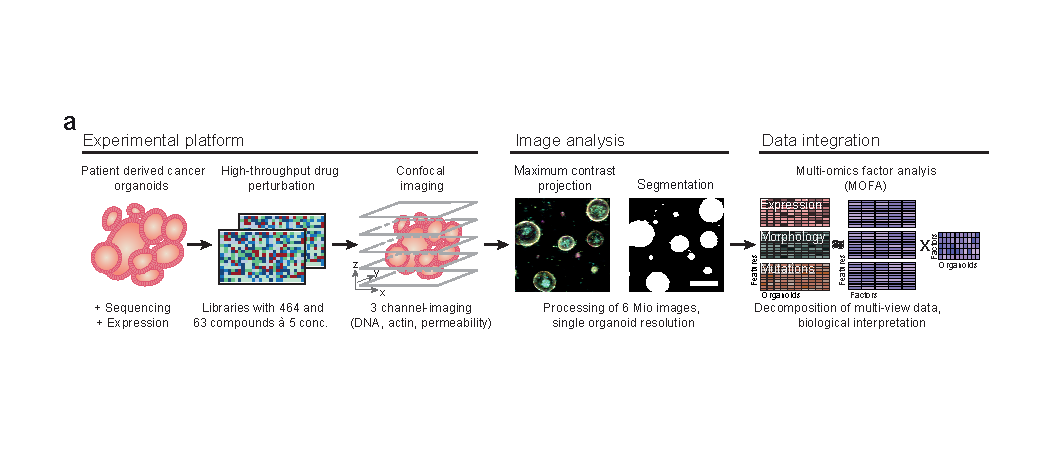
\includegraphics[width=\textwidth,
                height=\textheight,
                keepaspectratio]{figures/promise/pdf/fig_1_1.pdf}
\caption[Overview of multi-view profiling experiments]{\textbf{Overview of multi-view profiling experiments a} Organoids were isolated from endoscopic biopsies from patients with colorectal cancer. Organoids were dissociated and evenly seeded in 384-well plates before perturbation with an experimental (464 compounds) and a clinical compound library (63 compounds à 5 concentrations, 842 perturbations across both libraries). After treatment, high-throughput fluorescence microscopy was used to capture the morphology of organoids.  The multi-channel (DNA, beta-actin, cell permeability) 3D imaging data was projected, segmented, and descriptive features were extracted to quantify potential drug-induced phenotypes. Untreated organoid morphology, organoid size and drug activity scores were integrated with mRNA expression and mutation data in a Multi-Omics Factor Analysis (MOFA) to increase interpretability of organoid variation. Figure created with support from Johannes Betge (graphical presentation) and adapted from \textit{The drug-induced phenotypic landscape of colorectal cancer organoids} \citep{Betge2022-kr}}
\label{fig_130}
\end{figure}

Patient derived organoids (PDOs) are physiological 3D tumor models that can be efficiently derived from cancer and normal tissues.1–3 Organoid isolation from human primary tumors and metastases1,4 has enabled the establishment of living biobanks.2,3,5–7 Notably, patient derived organoids have been shown to represent their origin’s molecular features and morphology,2–4,8 enabling functional experiments such as drug testing ex vivo.3,5,9–14 
Image-based profiling is a high-throughput microscopy-based methodology to systematically measure phenotypes of in vitro models. By learning a lower dimensional representation of biological images, biological states can be described, quantified and deciphered. When scaled and combined with chemical or genetic perturbations, this becomes a powerful approach to gain systematic insights into biological processes, making it a popular method in drug discovery and functional genomics research.15–17. Image-based assays have for instance been used to screen large libraries of small molecules to identify potential drug candidates, to analyze a drugs mode of action, or to classify drug-gene interactions by cell-morphology.18–21 Recently, image-based profiling of monogenic disease models has been particularly relevant for drug discovery. Here, primary cells from diseased tissue are profiled, perturbed and candidate drugs reversing the phenotype from a diseased to a healthy cell morphology are prioritized for drug development or used as diagnostics.22,23
Previously, high-throughput image-based profiling experiments have mostly been performed in a limited number of adherent cell lines and not been available to a growing number of disease models that require more sophisticated culture conditions, such as models from diverse cancers, rare genotypes or personalized disease models. Performing image-based profiling experiments of patient derived cancer organoids, a prime example for a complex 3D polygenic disease model, are, however, a technical and biological challenge. While image-based drug testing in organoids have been performed, the morphological heterogeneity of patient-derived cancer organoids between and within patient donors as well as their diverging behavior upon molecular perturbations are not yet systematically understood.24–26
Here we report on a large-scale image based phenotyping study of patient derived cancer organoids. We generated patient derived organoids from colorectal cancer patients and treated 11 organoid models with more than 500 experimental and clinically used compounds at different concentrations. We systematically mapped the morphological heterogeneity of patient derived organoids and their response to compound perturbations from more  than  3,700,000  confocal microscopy images. We identified a heterogeneous landscape of organoid phenotypes mainly driven by differences in organoid size, viability and cystic vs. solid organoid architecture. Using multi-omics factor analysis, we identified biological programs underlying these phenotypes and compounds that modulate them. For example, we linked cystic organoid architecture with a LGR5+ enriched, Wnt signaling dependent organoid state that could be induced via MEK inhibition and organoid size to an IGF-1R driven organoid state that was relatively insensitive to EGFR inhibition and could be induced via mTOR inhibition. A better understanding of organoid phenotypes and the ability to use multi-omics data to annotate organoid states and their plasticity have the potential to further accelerate image-based drug discovery for complex multigenic diseases.


\subsection{Identification of molecular factors of colorectal cancer organoid architecture and plasticity}

\subsection{Demonstrating Small Molecule Profiling in a multi-step, multi-view model of colon cancer initiation}
\end{flushleft}

% First, we isolated and characterized patient derived colorectal cancer organoids. Next, we performed high- throughput drug profiling of these organoids. Here, we observed a variety of recurring treatment-induced phenotypes. These were linked to specific cellular processes. Of note, the treatment response of organoids in-vitro matched the response of donating patients.

% Second, we isolated colon organoids from healthy mouse tissue. By using gene-editing, we generated models of colon adenoma - a precursor lesion of colorectal cancer. These models carried different combinations of mutations in the Apc and Kras gene. Both are frequent and co-occurring mutations in colorectal cancer (Schell et al. 2016). To better understand the mechanisms of tumor development, we performed a multi- omics characterization in these adenoma models. Moreover, we profiled genotype specific drug effects. Here we found a reorganization of organoid phenotype after loss of Apc, which masks the effects of an isolated Kras mutation. Loss of Apc leads to genotype specific drug-induced phenotypes and vulnerabilities. Oncogenic Kras buffers a subset of these vulnerabilities, offering a new perspective on the relationship of Apc and Kras during tumor development.